\documentclass[a4paper]{article}
% standard packages
\usepackage{amssymb}
\usepackage{euscript}
\usepackage{eurosym}
\usepackage{graphicx}
\graphicspath{{img/}}
\usepackage{color}
\usepackage{epsfig}
\usepackage{fullpage}
\usepackage[colorlinks=true]{hyperref}
\usepackage{titling}

% title style
\pretitle{\noindent\LARGE}
\posttitle{\\[1ex]}
\preauthor{\large}
\postauthor{,}
\predate{\large(}
\postdate{)}
\date{last update: \today}

% large page size
\oddsidemargin -1cm
\topmargin -1cm
\textwidth 18cm
\textheight 27cm
\pagestyle{empty}


% PDF figure (floating)
\newcommand{\image}[3]{
\begin{figure}[#1]
\begin{center}
\caption{\small#3}
\includegraphics{img_#2.pdf}
\label{image:#2}
\end{center}
\end{figure}
}

% simple image
\newcommand\simpleimage[3][\linewidth]{
\smallskip\begin{center}\vbox{\noindent
\includegraphics[width=#1]{#2}\\%
\parbox{#1}{\it#3}}\end{center}
\medskip}

%\newcommand\simpleimage[3][\linewidth]{
%\smallskip\vbox{\noindent
%\includegraphics[width=#1]{#2}\\%
%\it#3}
%\medskip}


% companies
\def\SchaefferAG{\href{https://www.schaeffer-ag.de/en/}{Schaeffer-AG}}
\def\MultiCB{\href{https://portal.multi-circuit-boards.eu}{Multi-CB}}
\def\BlueFors{\href{https://www.bluefors.com/}{BlueFors}}

\def\Ohmite{\href{https://www.ohmite.com}{Ohmite}}
\def\Firmetal{\href{http://www.firmetal.com}{Firmetal}}
\def\Bruker{\href{https://www.bruker.com}{Brucker}}

% use this to refer to Farnell and RS numbers:
\def\FarnellN#1{\href{https://fi.farnell.com/#1}{Farnell:#1}}
\def\RSN#1{\href{https://fi.rsdelivers.com/productlist/search?query=#1}{RS:#1}}

% products:
\def\OhmiteOFOD{\href{https://www.ohmite.com/assets/docs/res_od_of_oa.pdf}{Ohmite OF/OD series}}

% Supplementary materials on github <report> <file>
\def\GitFile#1#2{\href{https://github.com/slazav/he3notes/raw/master/#1/#2}{#1/#2}}

% Supplementary materials on my users.aalt.fi page
\def\WWWFile#1{\href{https://users.aalto.fi/~zavyalv1/#1}{#1}}


%progams
\def\MagnettiProg{\href{https://github.com/slazav/magneetti}{\tt magnetti}}



\title{NMR magnet}
\author{V.Zavjalov}

\twocolumn
\begin{document}
\maketitle

NMR magnet for $^3$He experiments in DryDemag cryostat (summer 2016). The bottom flange
is connected to the nuclear demagnetization stage sinter volume. There is
a 6mm CuNi tube for soldering an experimental cell. The coil former is
thermally separated from the nuclear stage by Nb shield (Note: now the
lower part of the coil former is touching the shield. If one makes a
design with a gap there it will be much smaller heat leak through
niobium). The shield fully encapsulates the magnet. In the shield there
is a D6 hole for the cell leg, D3 and D4 screw holes near corners (where
marnetic field is small) and possible gap between Nb tube and top/bottom
plates.

\begin{center}
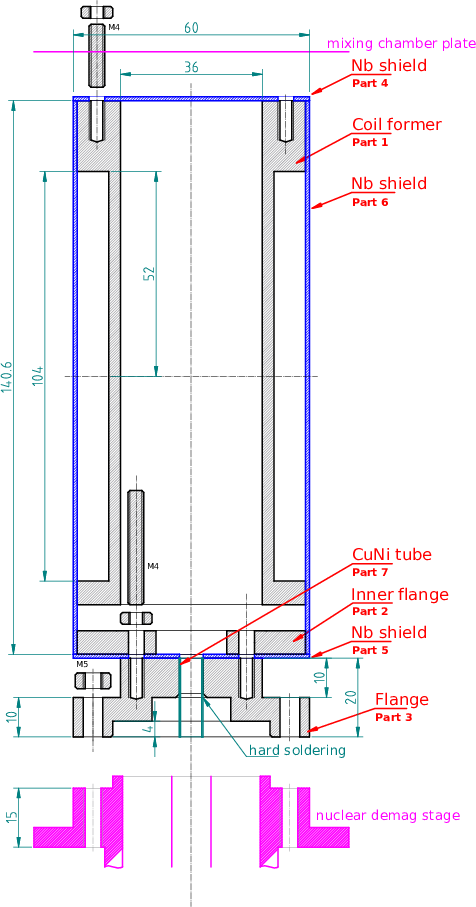
\includegraphics[width=6cm]{img/solenoid_plan.png}
\end{center}

\vbox{\noindent
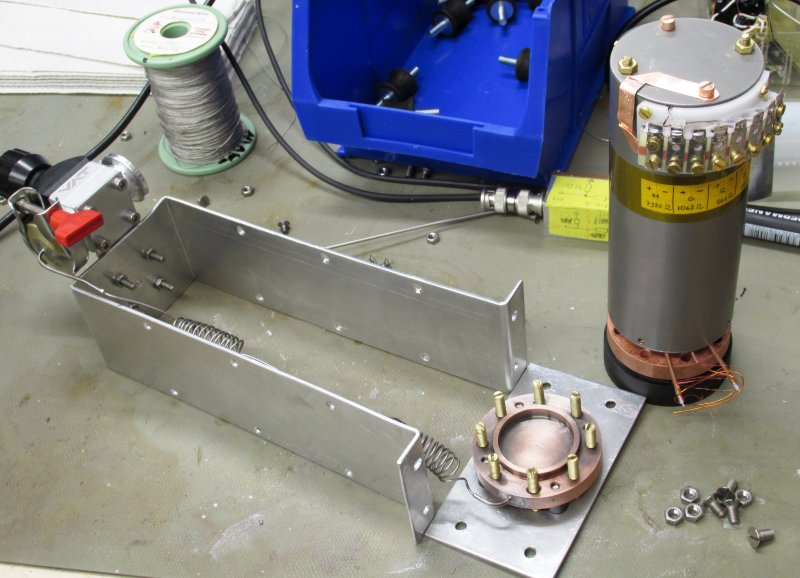
\includegraphics[width=\linewidth]{img/solenoid.jpg}\\
\it Solenoid and testing frame
}

The coil former and flanges have been made of oxigen-free copper in LTL
workshop and then annealed for 2 hours at 900$^\circ$C in
$2\cdot10^{-3}$~mbar of air (remove hidrogen, oxidize magnetic
impurities, anneal copper for better conductivity). Niobium parts have
been ordered in \Firmetal{} company (534\euro{} for the
$60\times1\times140$~mm tube, 153\euro{} for $65\times140\times1$~mm
plate).

All drawings: coil former, flanges, niobium shield, contact plate, testing flange:\\
\WWWFile{suppl/20161103-nmrmag/draw.zip}

\vbox{\noindent
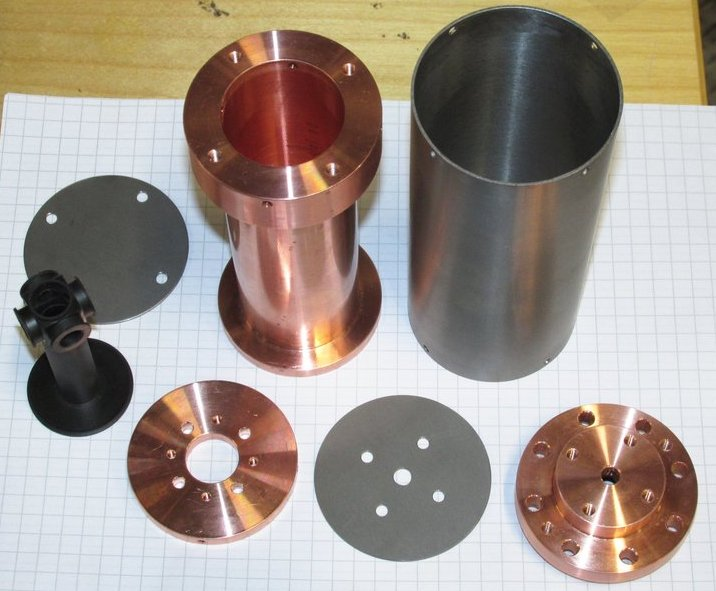
\includegraphics[width=\linewidth]{img/parts.jpg}\\
{\it parts}}
\vbox{\noindent
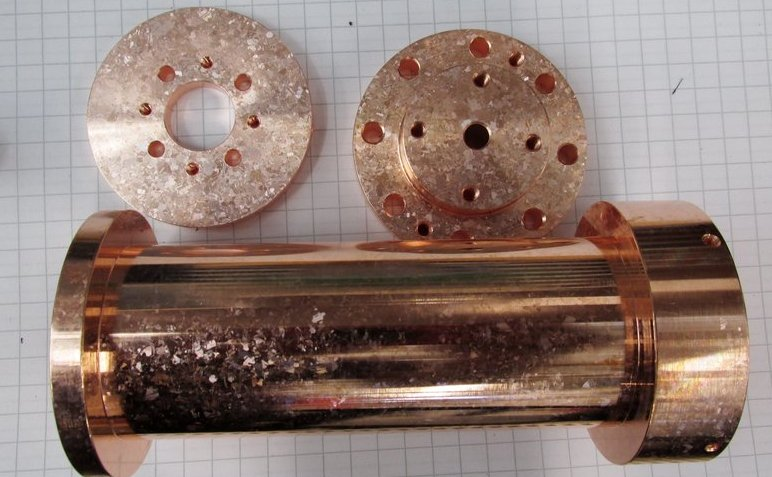
\includegraphics[width=\linewidth]{img/parts_ann.jpg}\\
{\it copper parts after annealing}}

\subsection*{Magnet calculation}
Coil calculations and optimisation have been done with \MagnettiProg{} program.\\
Optimization details:\\
\WWWFile{texts/2016-nmrmagcalc.pdf}\\
Script for optimization:\\
\WWWFile{suppl/2016-nmrmag/calc\_scr.zip}\\
Calculated field profiles (text table):\\
\WWWFile{suppl/2016-nmrmag/calc\_res.zip}

\vbox{\noindent
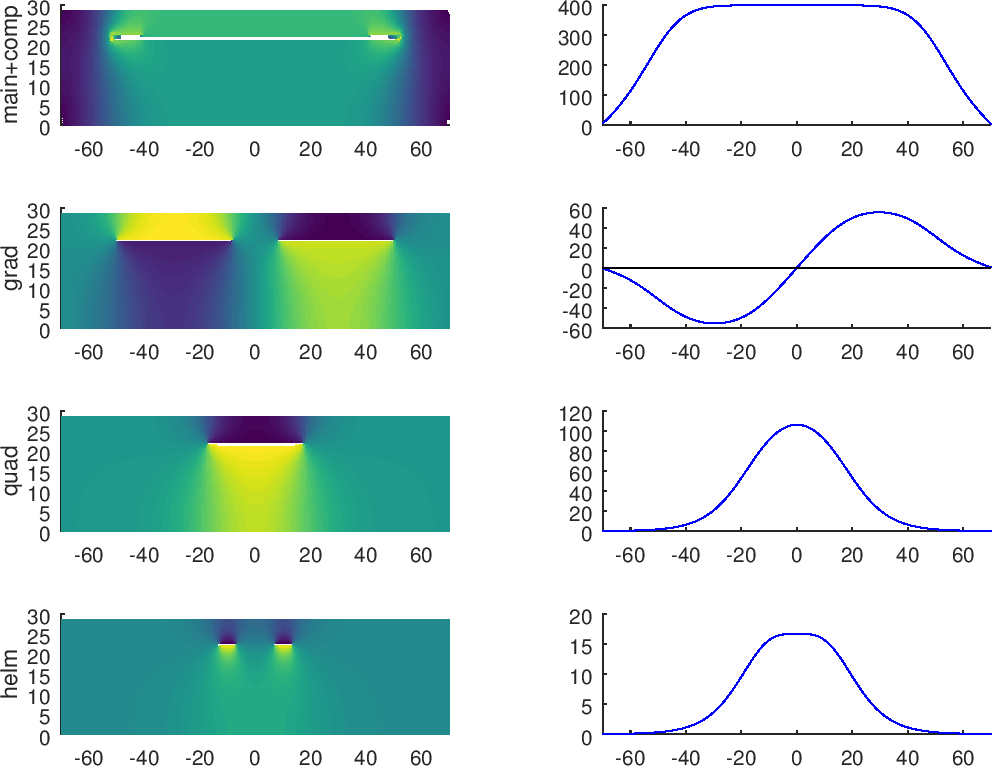
\includegraphics[width=\linewidth]{img/field_prof.png}\\
{\it calculated field profiles}}

\subsection*{Magnet winding}

Winding was done 20-21.9.2016. Before winding a plastic rod with
longitudinal grooves on the surface have been inserted in the coil former
to prevent its deformation. After winding it was removed by drilling.

{\bf Wire.} Vacryflux 5001. 54 NbTi filaments in Cu matrix; diameter:
$70\mu$m without isolation, $83-85\mu$m with isolation; Cu/NbTi ratio:
1.35/1; critical current: 2~A at 3~T, 1~A at 8~T; resistance at room
temperature $8.0\Omega/$m; bought from \Bruker. Stycast-1266 was used to
fill the coil.

\vbox{\noindent
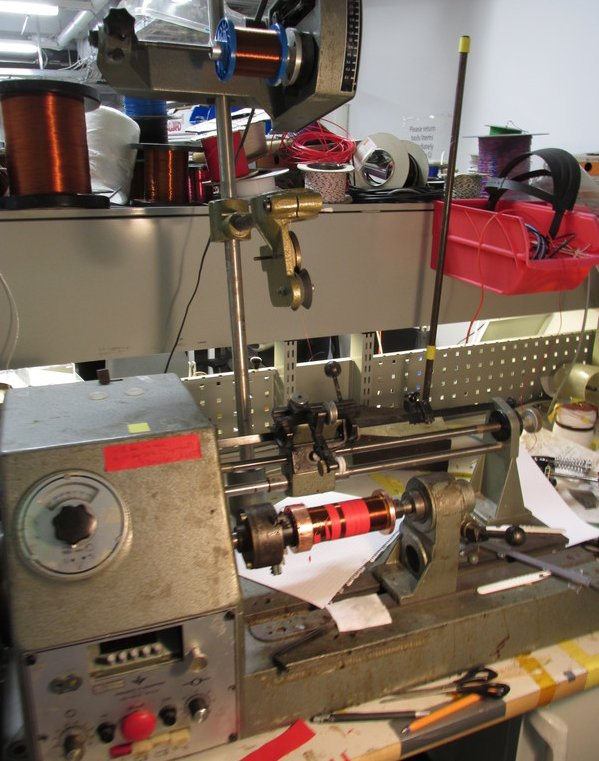
\includegraphics[width=\linewidth]{img/winding.jpg}\\
{\it winding process}}

{\bf Main coil:} length 104~mm, inner diameter 42~mm. Winding:
5 layers: 1208+1197+1200+1203+1193 turns. Accurate everywhere except
~4mm edges (hard to move from one layer to another with such a thin
wire). Then flatten edges with 12mm Kapton. Then 3 layers 11.2mm (compensation + 6thlayer):
140+97+120 turns. Then middle part of the 6th layer: 939 turns. Then
3 layers 11.2mm (compensation + 6thlayer): 133+103+133 turns.
Number of turns in the compensation coils is the same on both sides,
but it is a bit smaller then it should be.


{\bf Quadratic coil.} $L=34.8$, 2 layers, 408+408 turns.
After the coil had been made, the solenid was fully covered with Kopton
tape, and then by two layers of white paper to make a flat surface for
next coils.

{\bf Gradient coil.} Start at 2mm from solenoid edges, L=41.8mm R=~21.5
1 layer, 514+482 turns (not so accurate andassymetric).
Then the central part was covered with red "yellow" tape to make it flat
for the next coil.

{\bf Forth-power coil.} 1 layer, 79+79 turns, 6.8mm + 14mm gap + 6.0mm
(very assymetric for some reason).

\vbox{\noindent
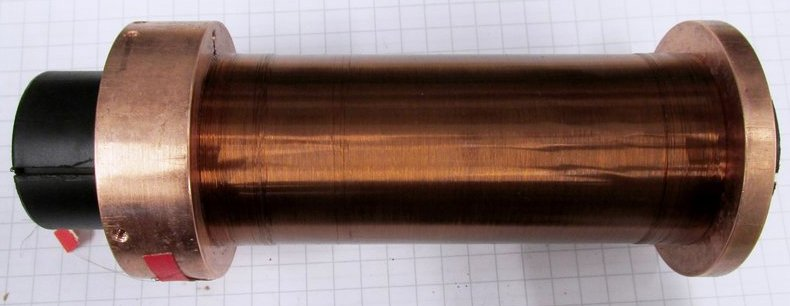
\includegraphics[width=\linewidth]{img/main_coil.jpg}\\
{\it main coil}}

\vbox{\noindent
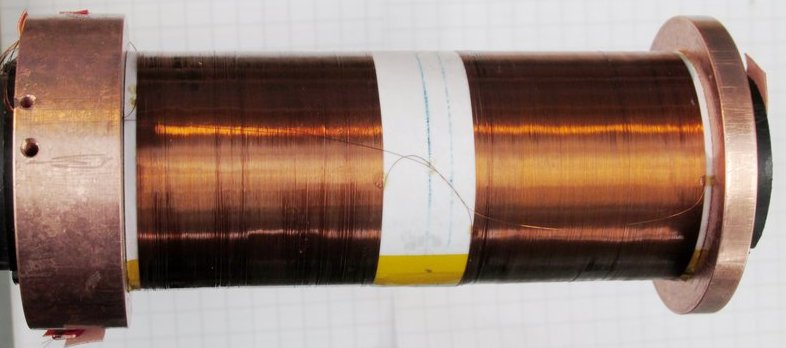
\includegraphics[width=\linewidth]{img/grad_coil.jpg}\\
{\it gradient coil}}

\vbox{\noindent
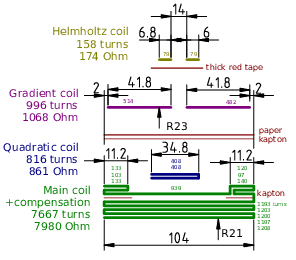
\includegraphics[width=\linewidth]{img/coil.png}\\
{\it coil layout}}

{\bf Connector:} plastic body + brass screws and nuts +
two-sided 0.4mm PCB (one side for contacts, another one for heat sink).
Wires are soldered to the connector at length 20-30cm (isolation was
removed in boiling NaOH).

\vbox{\noindent
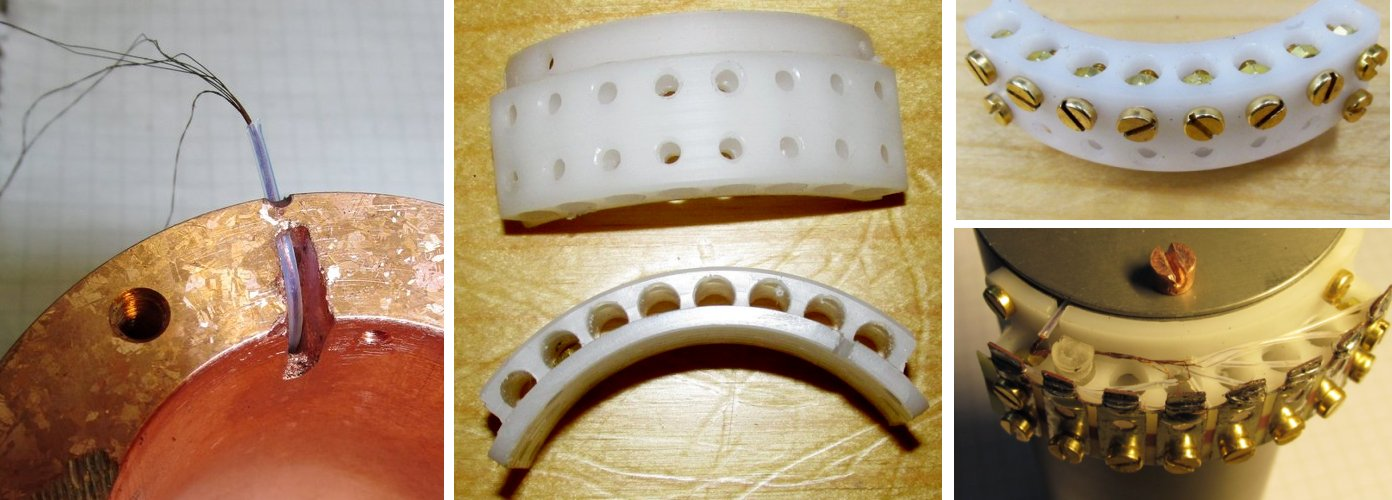
\includegraphics[width=\linewidth]{img/conn.jpg}\\
{\it connector}}
\medskip

\vbox{\noindent
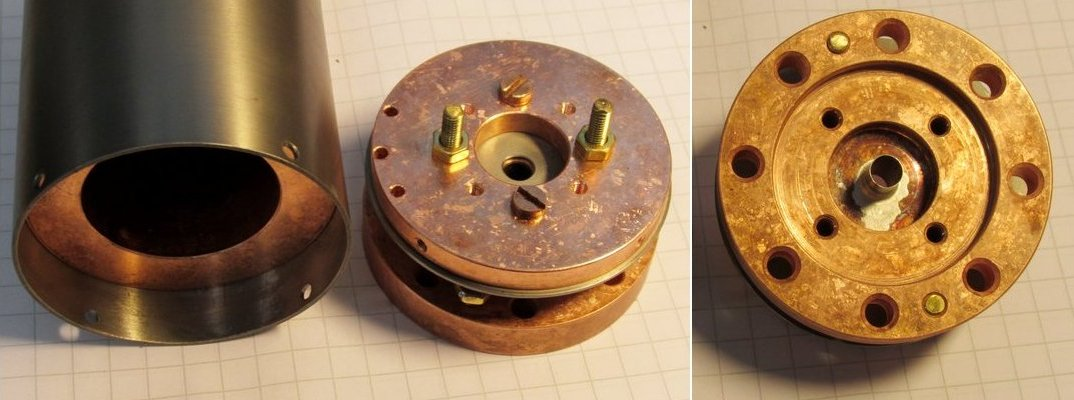
\includegraphics[width=\linewidth]{img/final.jpg}\\
{\it flanges}}

\subsection*{Solenoid parameters}

Field profile, calculated and measured by shift of $^3$He NMR line:

\medskip
\begin{tabular}{llll}
Coil  &  Field [G/A] vs r,z [cm] & measured\\\hline
Main   &  $397.996$                       & $407.72$\\
Grad   &  $31.4270\ z$                    & $1.43 + ? z$\\
Quad   &  $105.958 - 15.240 f_2$$^{(1)}$  & $108.27 - ? f_2$\\
Helm   &  $16.6512 - 1.0351 f_4$$^{(2)}$  & $18.09 - ? f_4$\\
\end{tabular}

\noindent
(1) $f_2 = z^2-r^2/2$\\
(2) $f_4 = z^4 - 3 z^2 r^2 + 3/8 r^4$
\medskip

For comparison, Rota quadratic coil in magnon condensate experiments was $2.231 - 3.304 f_2$


Errors, calculated in cylindrical volumes with length = diameter 10 and 20 mm,
and measured by normal $^3$He NMR line width.

\medskip
\begin{tabular}{llll}
Coil   & Err 20x20 & Err 10x10 & Err (measured) \\\hline
Main   & $1.4\cdot10^{-5}$ & $2.2\cdot10^{-6}$ & $\approx1\cdot10^{-4}$\\
Grad   & $1.5\cdot10^{-2}$ & $3.5\cdot10^{-3}$ & \\
Quad   & $4.9\cdot10^{-3}$ & $3.0\cdot10^{-4}$ & \\
Helm   & $1.8\cdot10^{-1}$ & $2.2\cdot10^{-1}$ & \\
\end{tabular}
\medskip

Coil resistances:

\medskip
\begin{tabular}{ll}\hline
Main: & 7980~$\Omega$\\
Grad: & 1068~$\Omega$\\
Quad: & 861~$\Omega$\\
Helm: & 174~$\Omega$\\
\end{tabular}
\medskip

On the connector all coils are shortened by 100~$\Omega$ resistors to
provide LR filtering.

\end{document}
